\documentclass[a4paper,12pt]{scrartcl}
\usepackage[utf8]{inputenc} 
\usepackage[T1]{fontenc}
\usepackage[english]{babel}
\usepackage{amsmath, amssymb,amsfonts}
\usepackage{graphicx}
\usepackage{csquotes}
\usepackage{geometry}
\usepackage{float}
\usepackage{framed, xcolor} 
\usepackage{scrlayer-scrpage}
\usepackage{siunitx}
\usepackage{subcaption}
\usepackage{chemgreek}
\usepackage{chemformula}
\usepackage[bookmarks,colorlinks=true]{hyperref}
\usepackage{booktabs}
% 1. ZUERST DIE VARIABLEN DEFINIEREN
\newcommand{\VERSUCHSDATUM}{March 20, 2026}
\newcommand{\PROTOKOLLDATUM}{\today}
\newcommand{\VerfasserEINS}{Julian Brügger}
\newcommand{\MatNoEINS}{3715444}
\newcommand{\EmailEINS}{st190050@stud.uni-stuttgart.de}
\newcommand{\StudiengangEINS}{B.Sc. Chemie}
\newcommand{\VerfasserZWEI}{Benedict Roßkopf}
\newcommand{\MatNoZWEI}{3718292}
\newcommand{\EmailZWEI}{st188124@stud.uni-stuttgart.de}
\newcommand{\StudiengangZWEI}{B.Sc. Simulation Technology}
\newcommand{\BETREUER}{}
\newcommand{\GRUPPENNR}{Gruppe X} % Darf nicht leer sein, wenn im Header genutzt
\newcommand{\VERSUCHSNR}{1}
\newcommand{\VERSUCHSNAME}{Molecular Dynamics}
% 2. DANN DAS LAYOUT
\geometry{left = 2.5cm, top = 3cm}
\renewcaptionname{english}{\figurename}{Fig.}
\renewcaptionname{english}{\tablename}{Tab.}
\sisetup{
    detect-weight=true, 
    detect-family=true,
    locale=UK,
    exponent-product = \cdot,
    separate-uncertainty=true,
    per-mode = symbol-or-fraction
}
\DeclareSIUnit{\angstrom}{\text{\AA}}
\hypersetup{
    colorlinks,
    linktocpage,
    citecolor=black,
    filecolor=black,
    linkcolor=black,
    urlcolor=black
}
\setlength{\parindent}{0 mm}
\setlength{\parskip}{2 mm} 
\pagestyle{scrheadings}
\clearpairofpagestyles % Löscht alte Voreinstellungen
\ihead{\VERSUCHSNR} 
\ofoot{\thepage} 
\begin{document}
\begin{titlepage}
\begin{center}
\Huge{\textbf{\VERSUCHSNAME}}\\
\vspace{10mm}
\Large{Protocol for the Computational Chemistry course by \\ \textbf{\VerfasserEINS\;\& \VerfasserZWEI }}\\
\vspace{10mm} 
\Large{University of Stuttgart}\\
\end{center}
\begin{center}
\begin{tabular}{ll}
\large{authors:}        & \large{\VerfasserEINS, \MatNoEINS} \\
& \large{\EmailEINS} \\
\vspace{2mm}\\
& \large{\VerfasserZWEI, \MatNoZWEI} \\
& \large{\EmailZWEI} \\                     
\vspace{0cm}\\
\large{date of experiment:} & \large{\VERSUCHSDATUM} \\
\vspace{0cm}\\
\large{submission date:} & \large{\PROTOKOLLDATUM}
\end{tabular}
\end{center}
\end{titlepage}

\section{Introduction}
In this exercise, we will perform a molecular dynamics (MD) simulation of a system of particles. This means that the time-dependent movement of the particles is simulated by solving Newton's equations of motion.
For this approach the forces acting on the particles must be calculated in every time step. Because of the large number of particles in a typical MD simulation, it quickly becomes unfeasable to calculate the forces by quantum mechanical methods. Instead, we will use classical force fields, which are empirical potential energy functions that describe the interactions between the particles.
The potential used for the first part of this exercise is the TIP3P water model, which is a commonly used model for simulating water. It consists of three point charges (one for the oxygen atom and two for the hydrogen atoms) and a Lennard-Jones potential to describe the van der Waals interactions between the oxygen atoms.
For the second part, which focuses on a copper crystal, we used the EMT potential, which is a many-body potential that describes the interactions between metal atoms. It consists of a pairwise potential that describes the interactions between pairs of atoms and a many-body term that describes the interactions between three or more atoms.

\section{Theory}

\subsection{Equations of Motion and the Verlet Algorithm}
In molecular dynamics simulations, atoms move according to classical mechanics. The trajectory of each atom is governed by Newton's second law:
\begin{equation}
    \mathbf{F}_i = m_i \mathbf{a}_i = m_i \frac{\mathrm{d}^2 \mathbf{x}_i}{\mathrm{d}t^2},
\end{equation}
where $\mathbf{F}_i$ is the force on atom $i$, $m_i$ is its mass, $\mathbf{a}_i$ its acceleration, and $\mathbf{x}_i$ its position. To propagate the system in time, the second derivative is discretised using a finite time step $\Delta t$:
\begin{equation}
    \frac{\mathrm{d}^2 x_i}{\mathrm{d}t^2} \approx \frac{x_{i+1} - 2x_i + x_{i-1}}{(\Delta t)^2}.
\end{equation}
Solving for the position at the next time step yields the \emph{Verlet algorithm}:
\begin{equation}
    x_{i+1} = 2x_i - x_{i-1} + \frac{F}{m}(\Delta t)^2.
\end{equation}
The choice of $\Delta t$ is crucial: it must be small enough to accurately resolve the fastest vibrational modes of the system, yet the simulation must run for long enough to capture the physical process of interest. In practice, $\Delta t$ is typically chosen to be about one tenth of the shortest relevant vibrational period.

\subsection{Statistical Ensembles}
Depending on which thermodynamic quantities are held constant, different statistical ensembles are used:
\begin{itemize}
    \item \textbf{NVE (microcanonical):} The number of particles $N$, the volume $V$, and the total energy $E$ are conserved. The system is thermally isolated, so neither heat nor work is exchanged with the surroundings. The total energy $E = E_\mathrm{kin} + E_\mathrm{pot}$ is exactly conserved, while kinetic and potential energy fluctuate in an anticorrelated manner.
    \item \textbf{NVT (canonical):} The number of particles $N$, the volume $V$, and the temperature $T$ are held constant. This is achieved by coupling the system to a thermostat, which adds or removes kinetic energy to maintain a fixed average temperature. In this ensemble, the total energy fluctuates.
\end{itemize}

\subsection{Langevin Thermostat}
The Langevin thermostat realises the NVT ensemble by adding two additional terms to Newton's equation of motion:
\begin{equation}
    m_i \ddot{\mathbf{x}}_i = \mathbf{F}_i - \gamma m_i \dot{\mathbf{x}}_i + \boldsymbol{\xi}_i(t),
\end{equation}
where $\gamma$ is a friction coefficient that removes kinetic energy (damping), and $\boldsymbol{\xi}_i(t)$ is a random Gaussian force (noise) that injects energy to mimic thermal fluctuations. The balance between friction and noise keeps the average kinetic energy, and hence the temperature, at the target value.

\subsection{Force Fields}
\subsubsection{TIP3P Water Model}
The TIP3P (Transferable Intermolecular Potentials 3P) model represents each water molecule as a rigid body with three point charges: a negative charge on the oxygen atom and two positive charges on the hydrogen atoms. The intermolecular interactions consist of:
\begin{itemize}
    \item \textbf{Coulombic interactions} between all intermolecular pairs of point charges.
    \item \textbf{Lennard-Jones interactions} between oxygen atoms only, of the form
    \begin{equation}
        V_\mathrm{LJ}(r) = 4\varepsilon\left[\left(\frac{\sigma}{r}\right)^{12} - \left(\frac{\sigma}{r}\right)^6\right].
    \end{equation}
\end{itemize}
Because TIP3P treats the water molecule as rigid, all three internal degrees of freedom (two O--H bond lengths and the H--O--H angle) must be frozen using geometric constraints. Here this is achieved with the RATTLE algorithm (Lagrange-multiplier-type constraints on bond lengths), implemented via the \texttt{FixBondLengths} class in ASE.

\subsubsection{EMT Potential for Copper}
The Effective Medium Theory (EMT) potential is a many-body empirical potential suited for transition metals. The total energy is written as a sum over atomic embedding energies that depend on the local electron density, supplemented by pairwise repulsive terms. Unlike pair potentials, EMT correctly describes the cohesive energy and elastic properties of FCC metals such as copper.

\subsection{Periodic Boundary Conditions}
In a finite simulation box, atoms near the boundary would experience unrealistic surface effects. Periodic boundary conditions (PBC) eliminate this by replicating the simulation box in all three spatial directions, so that atoms leaving one face immediately re-enter from the opposite face. The minimum image convention ensures that each atom interacts only with the nearest periodic image of every other atom.

\section{Results and Discussion}

\subsection{Water: Initial Geometry}
The experimental density of liquid water at \SI{20}{\celsius} is \SI{0.9982}{\gram\per\centi\metre\cubed}. From the mass of a single \ch{H2O} molecule and this density, the volume per molecule is
\begin{equation}
    V_\mathrm{mol} = \frac{m_\mathrm{H_2O}}{\rho \cdot N_A}.
\end{equation}
This yields a cubic box length of
\begin{equation}
    L_\mathrm{mol} = V_\mathrm{mol}^{1/3} = \SI{3.106}{\angstrom}
\end{equation}
per molecule. Replicating this unit cell $3\times3\times3$ times gives a simulation box of side length \SI{9.318}{\angstrom} containing 27 water molecules (81 atoms). Fig.~\ref{fig:water_unitcell} shows the geometry of one unit cell of the water model.

\begin{figure}[H]
    \centering
    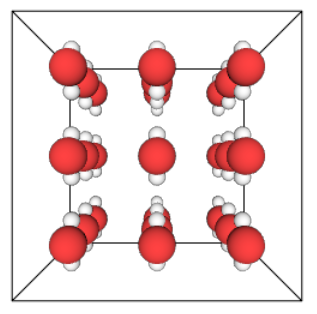
\includegraphics[width=0.4\textwidth]{water_init.png}
    \caption{Initial geometry of one unit cell of the TIP3P water model. The red sphere is the oxygen atom; the two white spheres are hydrogen atoms.}
    \label{fig:water_unitcell}
\end{figure}

This geometry was used as the starting point for an equilibration run in the NVT ensemble at \SI{300}{\kelvin} for \SI{500}{\femto\second} with a time step of \SI{2}{\femto\second}. The final configuration from this run was then used as the initial geometry for the subsequent NVE simulations.

\subsection{Water: NVE Energy Conservation}
Fig.~\ref{fig:water_NVE} shows the kinetic energy $E_\mathrm{kin}$, potential energy $E_\mathrm{pot}$, and total energy $E_\mathrm{tot} = E_\mathrm{kin} + E_\mathrm{pot}$ as a function of simulation time for an NVE run at $\Delta t = \SI{2}{\femto\second}$.

\begin{figure}[H]
    \centering
    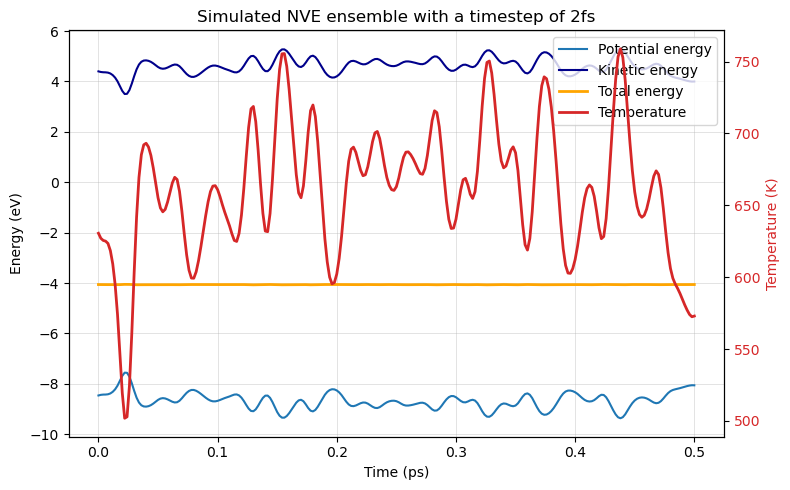
\includegraphics[width=0.85\textwidth]{NVE_2fs.png}
    \caption{Kinetic, potential, and total energy as a function of time in the NVE simulation of 27 water molecules at $\Delta t = \SI{2}{\femto\second}$.}
    \label{fig:water_NVE}
\end{figure}

In a perfectly isolated system (NVE ensemble), the total energy is an exact conserved quantity of Newton's equations of motion. The total energy therefore remains constant (or nearly so, limited only by numerical integration error). In contrast, kinetic and potential energy fluctuate in an anticorrelated fashion: when the molecules approach each other the potential energy rises while the kinetic energy falls, and vice versa. This exchange reflects the conversion between translational and interaction energy as the molecules vibrate and collide.

\subsection{Water: Effect of Time Step on Energy Conservation}

As the time step increases, the numerical integration error in the Verlet algorithm grows. For a time step of \SI{2}{\femto\second}, the total energy is well conserved throughout the simulation. At \SI{5}{\femto\second}, a noticeable drift and larger fluctuations appear, because the discretisation error is no longer negligible compared to the energy scale of the interatomic forces. At \SI{15}{\femto\second}, the time step exceeds roughly one tenth of the O--H stretching period , so the simulation can becomes unstable and the energy diverges.

Fig.~\ref{fig:water_NVE_comparison} illustrates the increasing energy drift for the three time steps.

\begin{figure}[H]
    \centering
    \begin{subfigure}[b]{0.4\textwidth}
        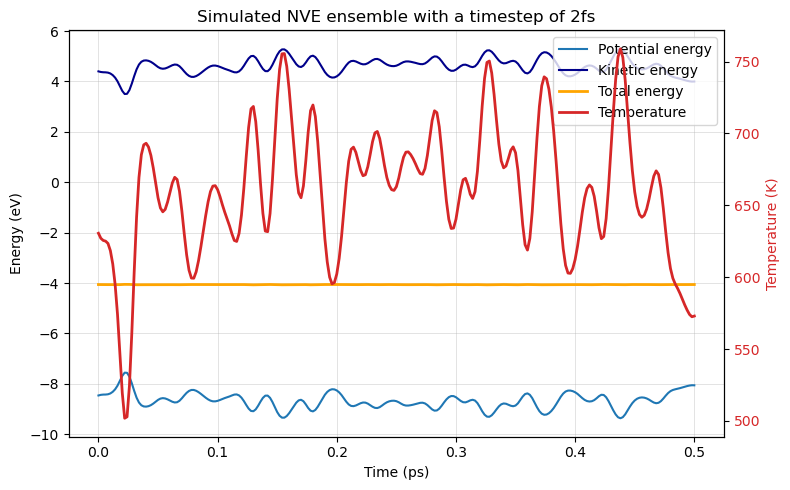
\includegraphics[width=\textwidth]{NVE_2fs.png}
        \caption{$\Delta t = \SI{2}{\femto\second}$}
    \end{subfigure}
    \hfill
    \begin{subfigure}[b]{0.4\textwidth}
        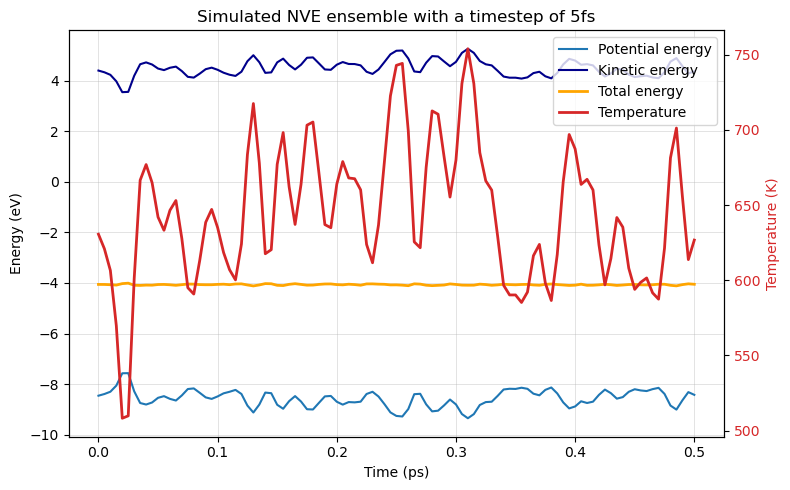
\includegraphics[width=\textwidth]{NVE_5fs.png}
        \caption{$\Delta t = \SI{5}{\femto\second}$}
    \end{subfigure}
    \caption{Total energy as a function of time in NVE simulations of 27 water molecules at three different time steps.}
    \label{fig:water_NVE_comparison}
\end{figure}

\subsection{Water: NVT Simulation with Langevin Thermostat}
Fig.~\ref{fig:water_NVT} shows the kinetic, potential, and total energy for a \SI{2}{\femto\second} simulation in the NVT ensemble at \SI{300}{\kelvin}.

\begin{figure}[H]
    \centering
    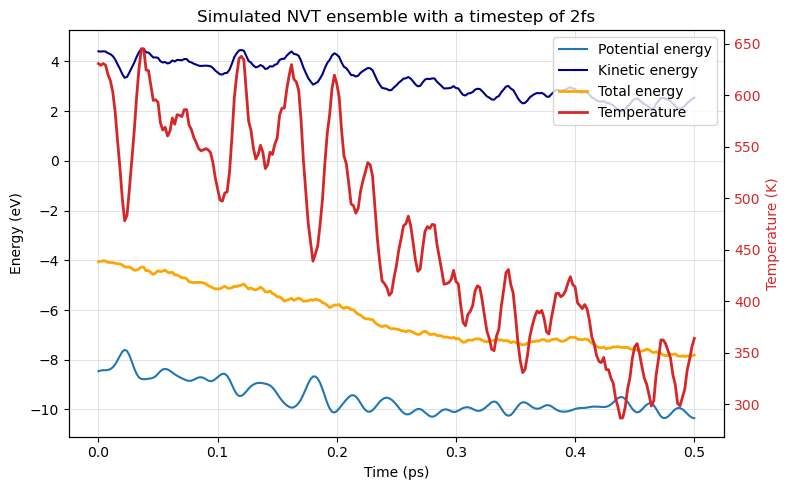
\includegraphics[width=0.85\textwidth]{NVT_2fs.png}
    \caption{Kinetic, potential, and total energy as a function of time in the NVT simulation of 27 water molecules at \SI{300}{\kelvin}, $\Delta t = \SI{2}{\femto\second}$.}
    \label{fig:water_NVT}
\end{figure}

In the NVT ensemble, the Langevin thermostat continuously adds and removes energy to maintain the target temperature of \SI{300}{\kelvin}. As a result, neither the total energy nor the kinetic or potential energy is conserved; all three fluctuate around their mean values. The kinetic energy fluctuations are directly related to the temperature fluctuations, while the total energy fluctuations reflect the heat exchanged with the (virtual) heat bath. Comparing with the NVE case, the kinetic energy is now more tightly controlled around its mean value (corresponding to \SI{300}{\kelvin}), whereas the total energy is no longer conserved.

\subsection{Copper: Vibrations at \SI{300}{\kelvin}}
A $5\times5\times5$ FCC supercell of copper was simulated in the NVT ensemble at \SI{300}{\kelvin} with the EMT potential and a time step of \SI{2}{\femto\second}. Fig.~\ref{fig:copper_distance_300K} shows the distance between two nearest-neighbour copper atoms as a function of simulation time.

\begin{figure}[H]
    \centering
    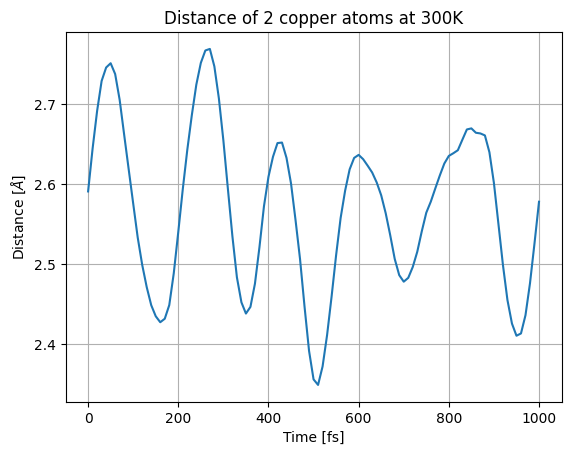
\includegraphics[width=0.8\textwidth]{distance_300K.png}
    \caption{Distance between two nearest-neighbour copper atoms as a function of time at \SI{300}{\kelvin}.}
    \label{fig:copper_distance_300K}
\end{figure}

The distance oscillates around the equilibrium nearest-neighbour separation in FCC copper. The vibrational peaks were identified at approximately $t = \SI{50}{\femto\second},\, \SI{270}{\femto\second},\, \SI{430}{\femto\second},\, \SI{600}{\femto\second},$ and $\SI{850}{\femto\second}$. From these, the average period of one full vibration cycle is:
\begin{equation}
    T = \SI{200}{\femto\second}.
\end{equation}
The corresponding vibrational frequency in wavenumber units is:
\begin{equation}
    \tilde{\nu} = \frac{1}{c \cdot T} = \frac{\SI{33356}{\centi\metre\per\second}}{\SI{200}{\femto\second}} \approx \SI{167}{\per\centi\metre}.
\end{equation}

The relatively low vibrational frequency of copper (compared to, for example, O--H stretching in water at $\approx\SI{3400}{\per\centi\metre}$, corresponding to a period of $\approx\SI{10}{\femto\second}$) is a direct consequence of the large atomic mass of copper ($m_\mathrm{Cu} \approx \SI{64}{\atomicmassunit}$) and the relatively soft metallic bonding. A vibrational period of \SI{200}{\femto\second} means that a time step of \SI{2}{\femto\second} corresponds to only $1\%$ of the period -- well within the accuracy requirement. In the TIP3P water simulation, the slowest modes (librations and hindered translations) are faster, but critically the constrained O--H stretch has a period of only $\sim\SI{10}{\femto\second}$, making \SI{2}{\femto\second} barely safe and \SI{15}{\femto\second} inappropriate. Thus, a larger time step is justified for copper than for water.

\subsection{Copper: Melting at \SI{1500}{\kelvin}}
At \SI{1500}{\kelvin}, which is above the experimental melting point of copper (\SI{1358}{\kelvin}), the crystal melts during the simulation. This is immediately visible in the trajectory: whereas at \SI{300}{\kelvin} the atoms undergo small oscillations around their equilibrium lattice positions, at \SI{1500}{\kelvin} they undergo large, diffusive displacements and lose their long-range order. The crystal structure collapses and the system transitions to a liquid-like disordered state.

Importantly, the \SI{1500}{\kelvin} simulation was performed without periodic boundary conditions (PBC). This is necessary because the standard periodic box enforces a fixed volume that was optimised for the FCC crystal at low temperature. With PBC active, the melting liquid would be constrained to that volume, leading to unphysical pressures and artifacts. Without PBC, the atoms are free to expand and rearrange as the crystal disorders.

Fig.~\ref{fig:copper_distance_1500K} shows the distance between the same two atoms as in the \SI{300}{\kelvin} simulation, now at \SI{1500}{\kelvin}.

\begin{figure}[H]
    \centering
    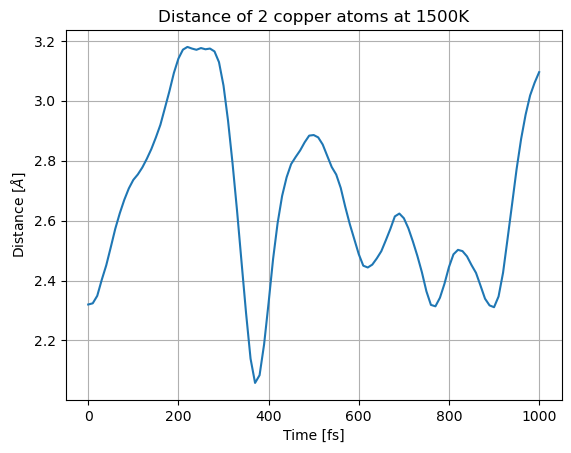
\includegraphics[width=0.8\textwidth]{distance_1500K.png}
    \caption{Distance between two initially nearest-neighbour copper atoms as a function of time at \SI{1500}{\kelvin}.}
    \label{fig:copper_distance_1500K}
\end{figure}

At \SI{1500}{\kelvin}, the distance between the two atoms increases strongly and irregularly over the course of the simulation, reflecting the diffusive motion of atoms in the liquid phase. The regular, periodic oscillations seen at \SI{300}{\kelvin} are replaced by larger, erratic fluctuations, consistent with the loss of the crystalline lattice. The peaks identified in the trajectory occur at $t = \SI{220}{\femto\second},\, \SI{250}{\femto\second},\, \SI{270}{\femto\second},\, \SI{500}{\femto\second},\, \SI{690}{\femto\second},$ and \SI{820}{\femto\second}, giving a mean apparent period of approximately \SI{120}{\femto\second} and a corresponding wavenumber of
\begin{equation}
    \tilde{\nu}_{1500\,\mathrm{K}} = \frac{\SI{33356}{\centi\metre\per\second}}{\SI{120}{\femto\second}} \approx \SI{278}{\per\centi\metre}.
\end{equation}
However, unlike at \SI{300}{\kelvin}, these peaks do not correspond to true harmonic vibrations around fixed lattice sites. The atoms are diffusing through the liquid, and the apparent periodicity in the distance is a consequence of transient nearest-neighbour cage dynamics in the melt, not long-lived crystal vibrations. The large and growing separation between the two originally adjacent atoms confirms that the crystal has melted.

\end{document}